% !TEX program  = xelatex
\documentclass{thxythesis}
% 中文题目
\title{多功能温湿度数字显示及控制系统的研制}
% 英文题目
\englishtitle{On the Research and Development of Multi-function Temperature - Humidity Monitor and Display System}
% 二级学院
\institute{}
% 专业
\major{计算机科学与技术}
% 姓名
\authorname{张\quad 三}
% 学号
\studentid{**************}
% 指导教师
\teachername{李\quad 四}
% 年月
\thesisdate{2019}{5}

\begin{document}
% 载入封面和诚信声明
\makecoverandfaith

% 中文摘要内容
\begin{Abstract}
本设计系统地设计了集温度与湿度采集、控制范围设置、声光报警、环境温湿度调节及液晶显示等多功能的实时控制系统。经过多次运行与检测,实践证明该电路工作稳定,显示清晰。本设计思路明晰,可拓展空间大。其可广泛\upcite{1}适用于与人民日常生活、工农业生产有关的温湿度测量以及加热制冷设备控制。

\keywords{温度;湿度;单片机;液晶显示屏}
\end{Abstract}

% 英文摘要内容
\begin{Abstract}[e]
The design is a multi-function real time monitor system which integrates functions like collecting temperature and humidity data, setting the limited digit scope, sound-light siren, as well as moderating the environmental temperature and humidity. Withstanding numerous trials and examinations, the circuit proves to be able to operate stably with a clear display. The idea of this design  is easy to understand and has great respect to develop. And it can be widely used in daily life and industry to measure the temperature and humidity as well as controlling the heating and cooling device.

\keywords[e]{emperature; Humidity; Monolithic Integrated Circuit}
\end{Abstract}

% 目录
\contents

% 第一层
\chapter{总体方案论述}
% 第二层
\section{总体功能及性能指标}
% 第三层
\subsection{总体功能}
% 第四层
\subsubsection{温度和湿度采集}
对爱情的渴望,对知识的追求,对人类苦难不可遏制的同情心,这三种纯洁但无比强烈的激情支配着我的一生。这三种激情,就像飓风一样,在深深的苦海上,肆意地把我吹来吹去,吹到濒临绝望的边缘。

我寻求爱情,首先因为爱情给我带来狂喜,它如此强烈,以致我经常愿意为了几小时的欢愉而牺牲生命中的其他一切。我寻求爱情,其次是因为爱情解除孤寂——那是一颗震颤的心,在世界的边缘,俯瞰那冰冷死寂、深不可测的深渊。我寻求爱情,最后是因为在爱情的结合中,我看到圣徒和诗人们所想象的天空景象的神秘缩影。这就是我所寻求的,虽然它对人生似乎过于美好,然而最终我还是得到了它。

我以同样的热情寻求知识,我希望了解人的心灵。我希望知道星星为什么闪闪发光,我试图理解毕达哥拉斯的思想威力,即数字支配着万物流转。这方面我获得一些成就,然而并不多。

爱情和知识,尽可能地把我引上天堂,但同情心总把我带回尘世。痛苦的呼号的回声在我心中回荡,饥饿的儿童,被压迫者折磨的受害者,被儿女视为可厌负担的无助的老人,以及充满孤寂、贫穷和痛苦的整个世界,都是对人类应有生活的嘲讽。我渴望减轻这些不幸,但是我无能为力,而且我自己也深受其害。

这就是我的一生,我觉得它值得活。如果有机会的话,我还乐意再活一次。


\subsubsection{风度测算}


\subsection{性能指标}
我以同样的热情寻求知识,我希望了解人的心灵。我希望知道星星为什么闪闪发光,我试图理解毕达哥拉斯的思想威力,即数字支配着万物流转。这方面我获得一些成就,然

爱情和知识,尽可能地把我引上天堂,但同情心总把我带回尘世。痛苦的呼号的回声在我心中回荡,饥饿的儿童,被压迫者折磨的受害者,被儿女视为可厌负担的无助的老人,以及充满孤寂、贫穷和痛苦的整个世界,都是对人类应有生活的嘲讽。我渴望减轻这些不幸,但是我无能为力,而且我自己也深受其害。

这就是我的一生,我觉得它值得活。如果有机会的话,我还乐意再活一次。

% 第五层格式和正文一样了,就不自动编号了

\section{系统组成及设计思路}


\chapter{硬件电路的设计}
温度模块使用...如图\ref{fig:sub-1}所示。...如图\ref{fig:sub-2}所示。

\begin{figure}[!h]
    \begin{subfigure}{0.45\linewidth}
        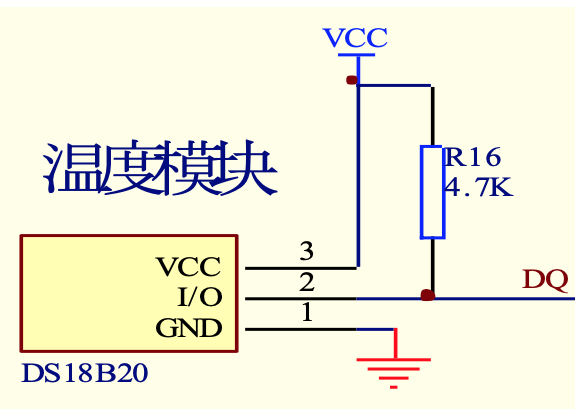
\includegraphics[scale=0.6]{static/1.png}
        \subcaption{温度采集电路}
        \label{fig:sub-1}
    \end{subfigure}
    \begin{subfigure}{0.5\linewidth}
        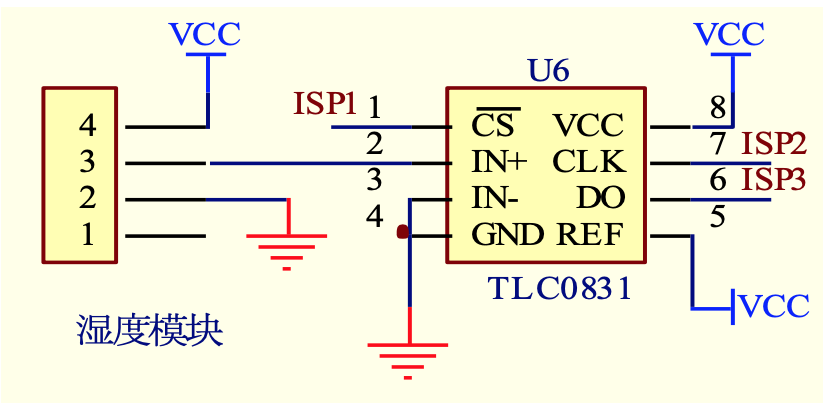
\includegraphics[scale=0.6]{static/2.png}
        \subcaption{湿度采集电路}
        \label{fig:sub-2}
    \end{subfigure}
    \centerline{\note{此图中的..................}}
    \caption{XXX图}
    \label{fig:circuit-diagram}
\end{figure}

\chapter{软件设计}

把........如下所示的数据表\ref{tab:t1}

\begin{Table}[!htbp]
\caption{实际湿度与测量湿度比较数据}
\label{tab:t1}
\begin{center}
\begin{tabular}{ p{2cm}<{\centering} |p{2cm}|p{2cm}|p{2cm}|p{2cm}|p{2cm}<{\centering}}
\hline
图号 & 实际湿度(\%RH)& 实际湿度的二进制 & 示波器测量湿度值 & 湿度十进制值(\%RH) & 误差 \\ \hline
(a) &  62  &  01011111  &  01011110   &   61  &  -1\\ \hline
(b) &  93  &  10001110  &  —  & —  & —\\ \hline
\end{tabular}
\end{center}
\end{Table}


% 参考文献
\begin{Reference}
\bibitem{1}金伟正编著.单线数字温度传感器的原理及应用[M].2000.6.
\bibitem{2}刘文涛.单片机语言C51典型应用设计[M].北京:人民邮电出版社,2005.
\bibitem{3}赵文博,刘文涛.单片机语言C51程序设计[M].北京:人民邮电出版社,2005.
\bibitem{4}李维缇,郭强编著.液晶显示应用技术[M].北京:电子工业出版社,2001.
\end{Reference}


% 致谢
\begin{Thanks}
本论文(设计)是在我的指导教师XXX副教授的亲切关怀和悉心指导下完成的。他严肃的科学态度,严谨的治学精神,精益求精的工作作风,深深地感染和激励着我。从题目的选择到最终完成,XXX老师都始终给予我细心的指导和不懈的支持。
\end{Thanks}

% 附录
\begin{Appendix}
\chapter{核心程序代码}
% 定制代码环境,敬请期待...

\begin{Table}[!h]
\caption{实际湿度与测量湿度比较数据}
\label{tab:t1-append}
\begin{tabular}{ p{2cm}<{\centering} |p{2cm}|p{2cm}|p{2cm}|p{2cm}|p{2cm}<{\centering}}
\hline
图号 & 实际湿度(\%RH)& 实际湿度的二进制 & 示波器测量湿度值 & 湿度十进制值(\%RH) & 误差 \\ \hline
(a) &  62  &  01011111  &  01011110   &   61  &  -1\\ \hline
(b) &  93  &  10001110  &  —  & —  & —\\ \hline
\end{tabular}
\end{Table}


\chapter{核武器制作指南}


如图 \ref{fig:sub-2-append} 所示,这就是一个测试~


\begin{figure}[H]
    \begin{subfigure}{0.45\linewidth}
        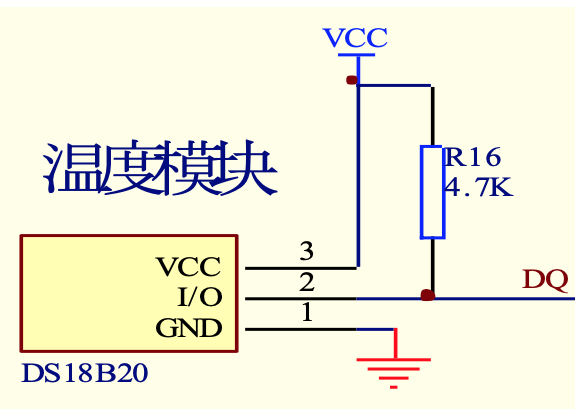
\includegraphics[scale=0.6]{static/1.png}
        \subcaption{温度采集电路}
        \label{fig:sub-1-append}
    \end{subfigure}
    \begin{subfigure}{0.5\linewidth}
        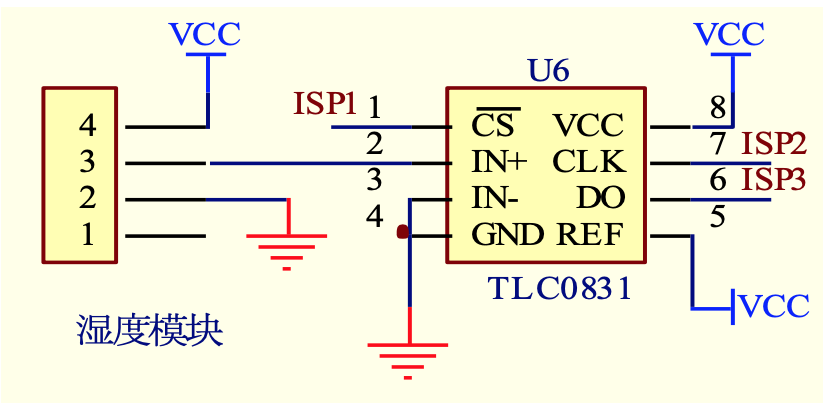
\includegraphics[scale=0.6]{static/2.png}
        \subcaption{湿度采集电路}
        \label{fig:sub-2-append}
    \end{subfigure}
    \centerline{\note{此图中的..................}}
    \caption{XXX图}
    \label{fig:circuit-diagram-append}
\end{figure}
\end{Appendix}


\end{document}